\chapter{Results}
At first, the result of a typical inpainting from the simple physical model is shown. After which the test results from the simple physical model and complex physical model are presented in their respective subchapters. An example of the inpainting of an ASPA is shown in Figure \ref{fig:inpainting_pixels}, which shows the real and inpainted pixel values. It is seen that the spectrum is correctly inpainted, there are no exceptional mismatches. Figure \ref{fig:inpainting_pixels_difference} shows the difference between each pixel. There is some noise visible on the inpainting, including a few >10\% outliers. But in general the inpainting is performed well.  Figure \ref{fig:real_inpainted_spectrum} shows both the inpainted and ground truth spectrum. Notice how the shape of the spectra mainly correspondent to each other, but the transit depth of several spectral bins are off. This is explained by the inpainted normalisation factors being different from the ground-truth values. Note that these plots solely visualise the performance of a single inpainting and do not give any information about the accuracy of the model. The ground truth and retrieved values of Figure \ref{fig:real_inpainted_spectrum} are visible in Table \ref{tab:single_simple_result}. Notice how the retrieved abundance of CO and the planet mass is a mismatch, while the other features appear to be a match. 

\begin{figure} [!htb]
    \centering
    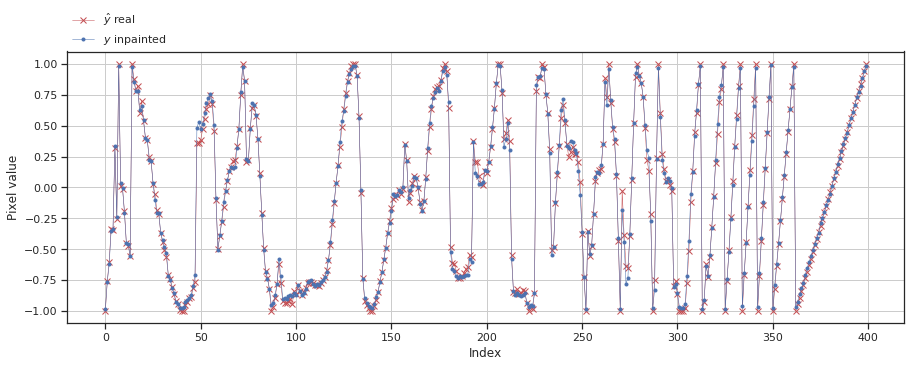
\includegraphics[scale=0.4]{figuren/real_inpainted_pixels.png}
    \caption{A visualisation of the ground truth and inpainted spectrum pixel values. Where 'Index' represents the index value of the respective pixel inside the spectrum block within the ASPA. Simplified, index 0-50 is the start ($\gtrapprox$0.3 $\mu$m) of the spectrum, where index 350-400 is the end of the spectrum ($\lessapprox$16 $\mu$m).}
    \label{fig:inpainting_pixels}
\end{figure}


\begin{figure} [!htb]
    \centering
    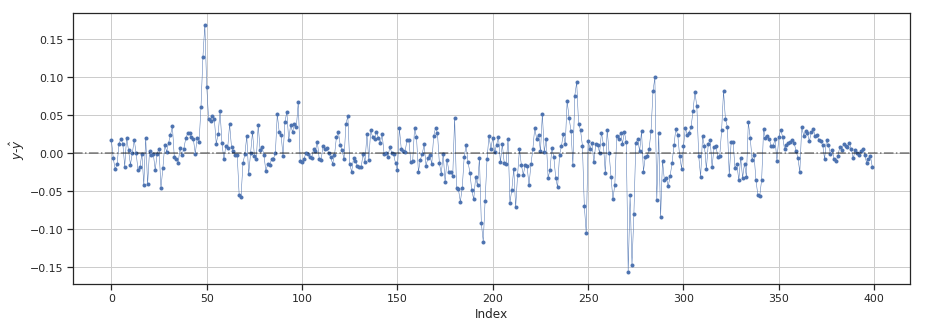
\includegraphics[scale=0.4]{figuren/real_inpainted_difference_pixels.png}
    \caption{The difference between the real and inpainted spectrum pixel values. }
    \label{fig:inpainting_pixels_difference}
\end{figure}

\begin{figure} [!htb]
    \centering
    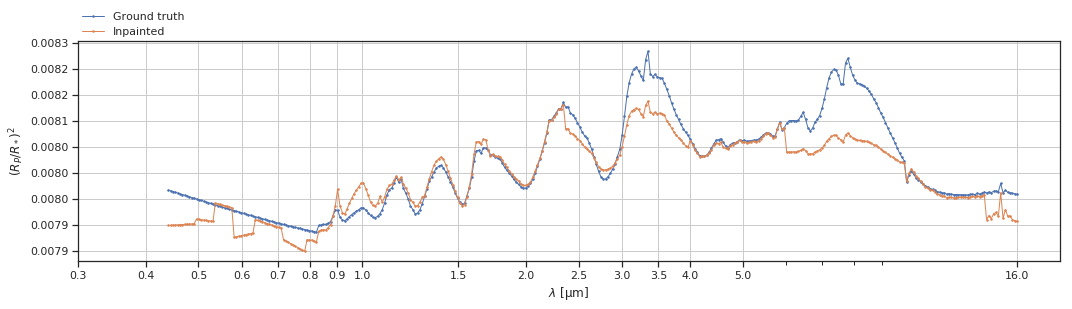
\includegraphics[scale=0.4]{figuren/real_inpainted.png}
    \caption{The ground truth and inpainted spectrum.}
    \label{fig:real_inpainted_spectrum}
\end{figure}

\begin{table}[!htb]
\centering
\caption{The retrieval result of a typical physically simple model.}
\label{tab:single_simple_result}
\begin{tabular}{|c|c|c|c|c|c|}
\hline
\textbf{Variable} & \textbf{ground truth} & \textbf{retrieved} & \textbf{absolute error} & \textbf{percentage error} \\ \hline
$\mathrm{H_2O}$               & -4.11                 & -3.74              & 0.37                    & -9.00                     \\ \hline
$\mathrm{CO_2}$               & -1.78                 & -1.41              & 0.37                    & -20.8                    \\ \hline
$\mathrm{CO}$                & -2.56                 & -5.53              & -2.97                   & 116                    \\ \hline
$\mathrm{CH_4}$               & -3.33                 & -3.36              & -0.03                   & 0.90                      \\ \hline
$M_p$                & 1.87 $\mathrm{M_J}$                  & 1.21 $\mathrm{M_J}$               & -0.66 $\mathrm{M_J}$                   & -35.3                    \\ \hline
$R_p$                & 1.27 $\mathrm{R_J}$                  & 1.28 $\mathrm{R_J}$               & 0.01 $\mathrm{R_J}$                    & 0.79                      \\ \hline
$T_p$                & 1890 K                  & 1780 K               & -110 K                    & -5.82                     \\ \hline
\end{tabular}
\end{table}






\section{Simple Physical Models}
Presented in this subchapter are the result of the simple physical model evaluation. The global percentage and absolute errors per feature are given in Table \ref{tab:simple_result}. Where $\Delta \overline{y} (\mu)$ is the mean absolute error, $\Delta \overline{y} (1\sigma)$ the one standard deviation absolute error, $\Delta \overline{y}_\% (\mu)$ the mean percentage error and $\Delta \overline{y}_\% (1\sigma)$ the one standard deviation percentage error. Notice how the errors on CO and CH$_4$ are relatively large compared to the other results. A visualisation of the predictions $y$ and ground-truth values $\hat{y}$ for the planet radius, CO and H$_2$O mixing ratios, including their mean and one standard deviation absolute error has been made in Figure \ref{fig:nac_plot}. Within this figure it is clear that SRON-GAN is able to predict the planet radius and H$_2$O mixing ratio, as long as the H$_2$O abundance is relatively high. The same goes for CO, but the errors in general are higher. 

\begin{table}[!htb]
\centering
\caption{The retrieval result of $3\cdot10^4$ physical simple models. Where }
\label{tab:simple_result}
\begin{tabular}{|c|c|c|c|c|}
\hline
\textbf{Feature} & \Delta \overline{y} (\mu) & \Delta \overline{y} (1\sigma) & \Delta \overline{y}_\% (\mu) & \Delta \overline{y}_\% (1\sigma) \\ \hline
H2O               & 0.039                        & 0.695                           & 1.448                          & 17.66                             \\ \hline
CO2               & 0.019                        & 0.596                           & 1.819                          & 23.29                             \\ \hline
CO                & 0.004                        & 1.918                           & 12.1                           & 74.54                             \\ \hline
CH4               & -0.225                       & 1.095                           & 13.55                          & 57.64                             \\ \hline
Mp                & 2.800$\cdot10^{-5}$ M$_J$                    & 0.498 M$_J$                       & 9.580                           & 41.91                             \\ \hline
Rp                & 0.494 R$_J$                        & 0.015 R$_J$                          & -0.369                         & 1.281                             \\ \hline
Tp                & 4.864 K                        & 455.1 K                          & 5.253                          & 33.01                            \\ \hline
\end{tabular}
\end{table}

\begin{figure} [!htb]
    \centering
    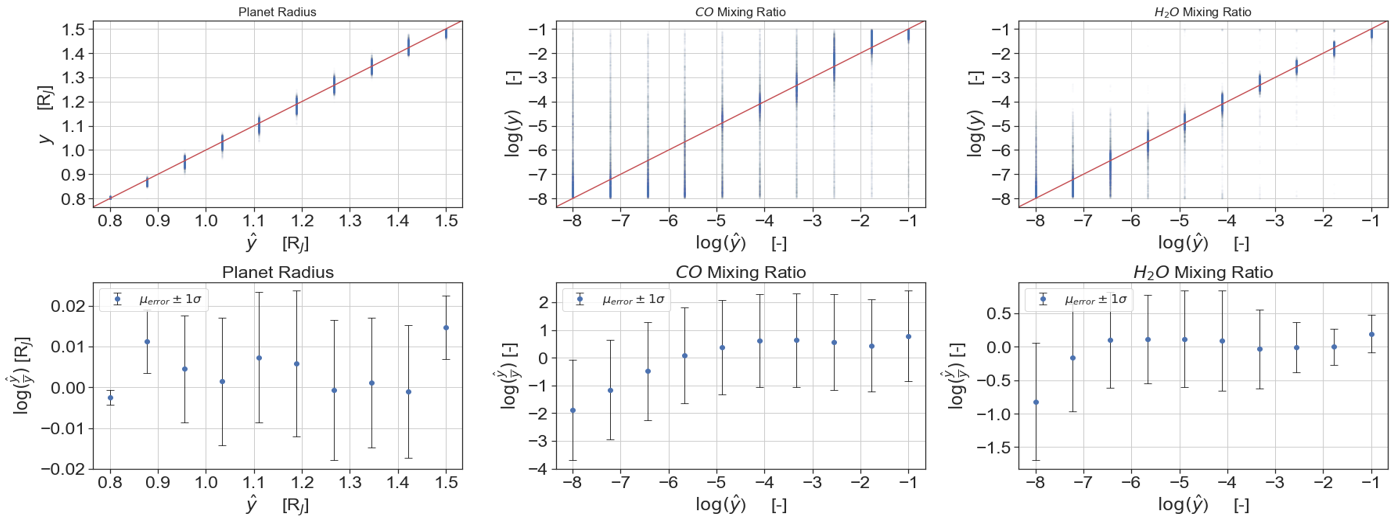
\includegraphics[width=\textwidth,keepaspectratio]{figuren/nacplot.png}
    \caption{The real versus inpainted features in the top row, where the red line describes the perfect predictions. The bottom row shows the mean and one standard deviation absolute error per unique ground truth value.}
    \label{fig:nac_plot}
\end{figure}

The contextual and perceptual percentage errors have been visualised in Figure \ref{fig:contextual_errors} and Figure \ref{fig:perceptual_errors}. Where the green area represents a $\pm$10\% margin. These plots visualise the importance of the ratio between the contextual and perceptual loss during inpainting. Figure \ref{fig:contextual_errors} shows that there is no increase in percentage error when the contextual loss becomes higher. Figure \ref{fig:perceptual_errors} shows that the value of the perceptual loss does not have a significant impact on the percentage errors per feature, except for CH$_4$. In general it is seen that the the contextual and perceptual loss are properly balanced.



\begin{figure} [!htb]
    \centering
    \includegraphics[width=\textwidth,height=\textheight,keepaspectratio]{figuren/complex y vs yhat.png}
    \caption{The real versus inpainted values per feature of the complex physical model, where the red line describes the perfect predictions.}
    \label{fig:complex_results_main}
\end{figure}


\section{Complex Physical Models}
This error analysis has been performed by the best performing GAN out of the four that have been traind. The results of the four GANs, that have been trained using the same conditions, are found in Figure \ref{fig:gan_results_small_gpu2} - \ref{fig:gan_results_small_gpu5}. Notice how there is a significant difference in the results. The GAN from Figure \ref{fig:gan_results_small_gpu3} seems to not have converged at all, while the GAN from Figure \ref{fig:gan_results_small_gpu4} has poorly converged.
A general visualisation for the predictions versus the ground-truth values is found in Figure \ref{fig:complex_results_main}. Notice how there are arrow like structures visible in e.g. CO, C$_2$H$_2$, C$_2$H$_4$, H$2$, HCN and He. It is to be noted that SRON-GAN gives a decent prediction for molecules with an exceptionally low abundance downwards to e.g. 10$^{-100}$ for C$_2$H$_2$ and 10$^{-70}$ for SO$_2$.
The predictions and their absolute errors are found in Figures \ref{fig:complex_results_1} - \ref{fig:complex_results_10}. Notice that in general for lower abundances the error bars become higher. This is expected, since the spectral signatures become significantly less visible. 
Finally, the result of the retrievals performed on real observations is presented in Table \ref{table:real_result}. The retrieval result of ARCiS is found in Table \ref{table:real_result_arcis}. Notice how SRON-GAN fails to predict the planet mass and half of the temperatures, but the other predictions are mostly in agreement with the retrieval results of ARCiS.

\begin{figure} [!htb]
    \centering
    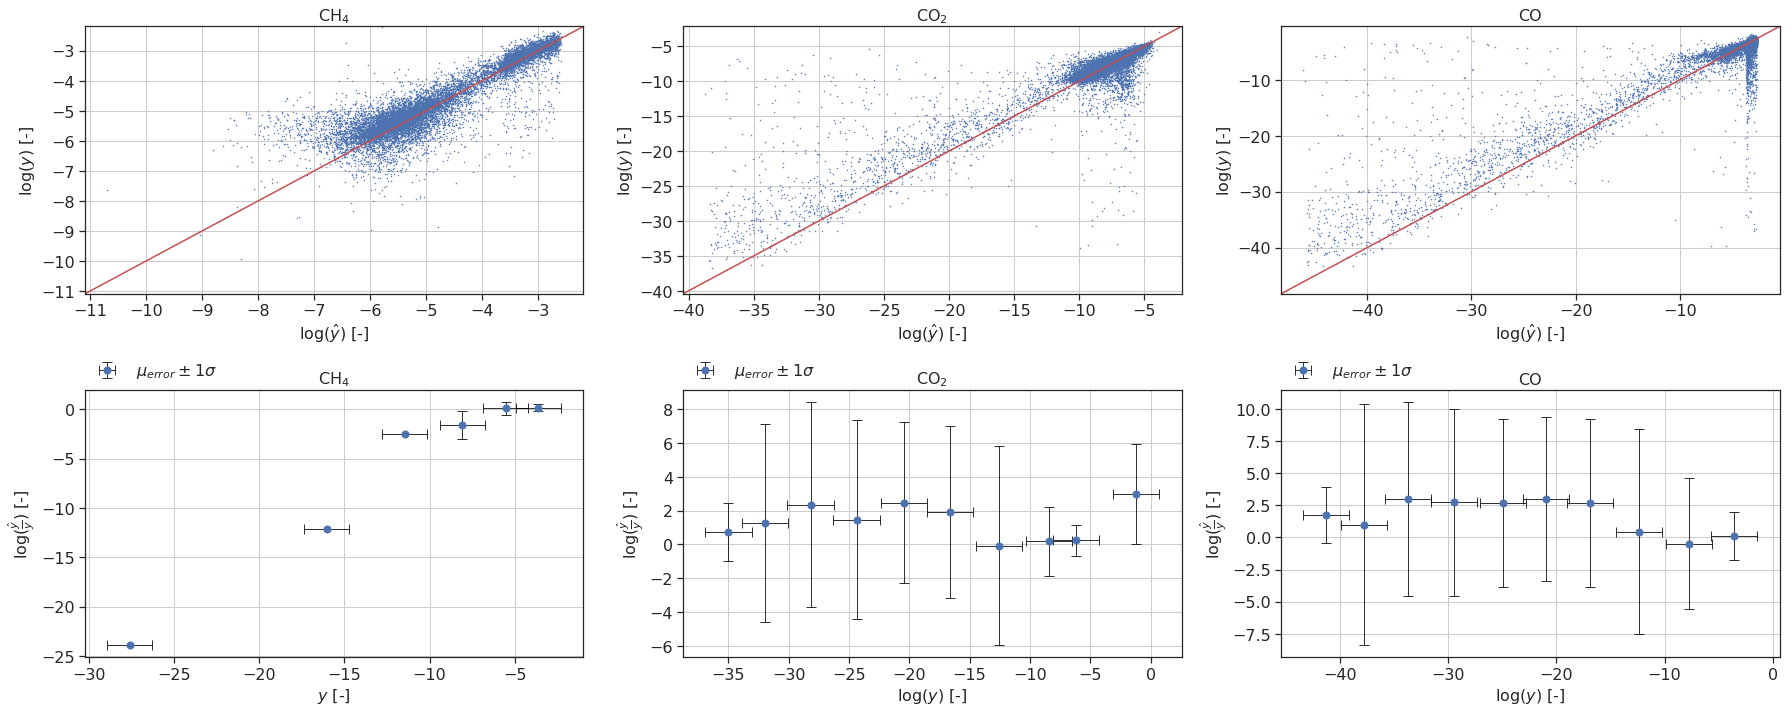
\includegraphics[width=\textwidth,keepaspectratio]{figuren/results1.png}
    \caption{The top row contains real versus inpainted values per feature of the complex physical model, where the red line describes the perfect predictions. Within the bottom row the mean and one standard deviation absolute errors are visualised. The horizontal error bar described the bin width, whereas the vertical error bar describes the one standard deviation error on the mean error of the bin. }
    \label{fig:complex_results_1}
\end{figure}

\begin{figure} [!htb]
    \centering
    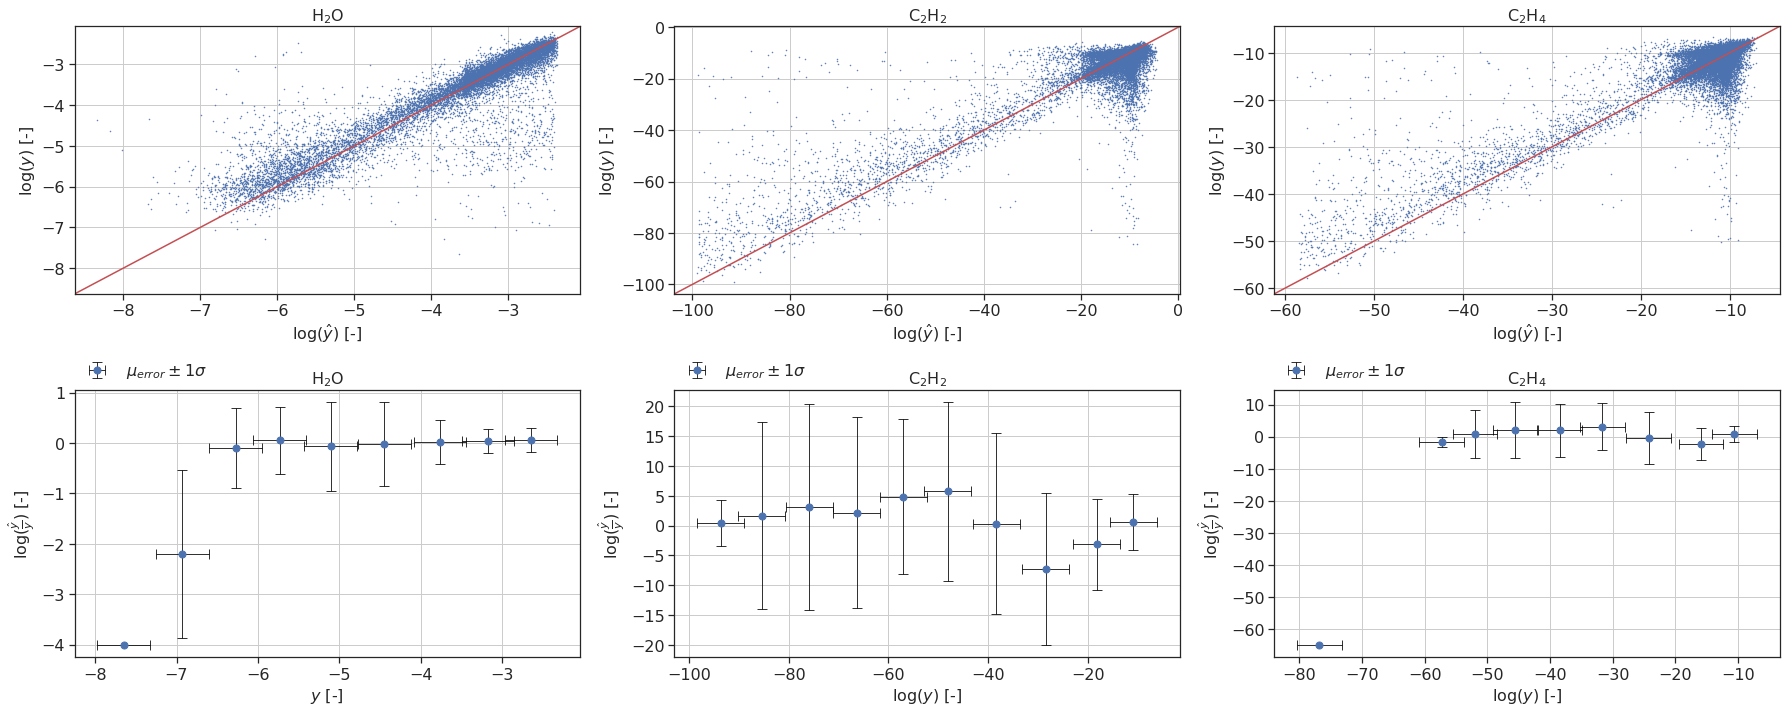
\includegraphics[width=\textwidth,keepaspectratio]{figuren/results2.png}
    \caption{Same as Figure \ref{fig:complex_results_1}.}
    \label{fig:complex_results_2}
\end{figure}

\begin{figure} [!htb]
    \centering
    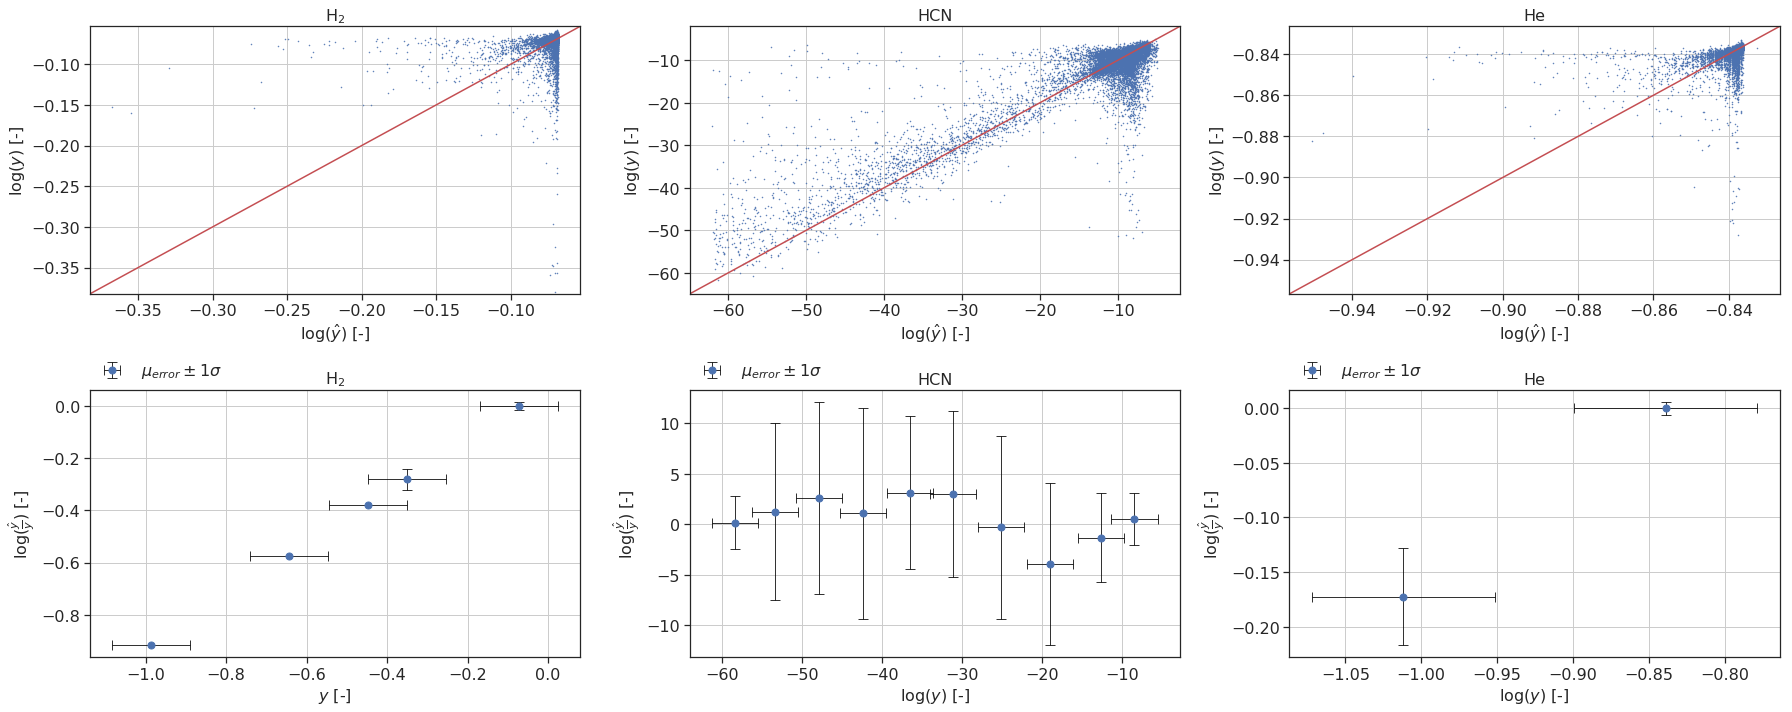
\includegraphics[width=\textwidth,keepaspectratio]{figuren/results3.png}
    \caption{Same as Figure \ref{fig:complex_results_1}.}
    \label{fig:complex_results_3}
\end{figure}

\begin{figure} [!htb]
    \centering
    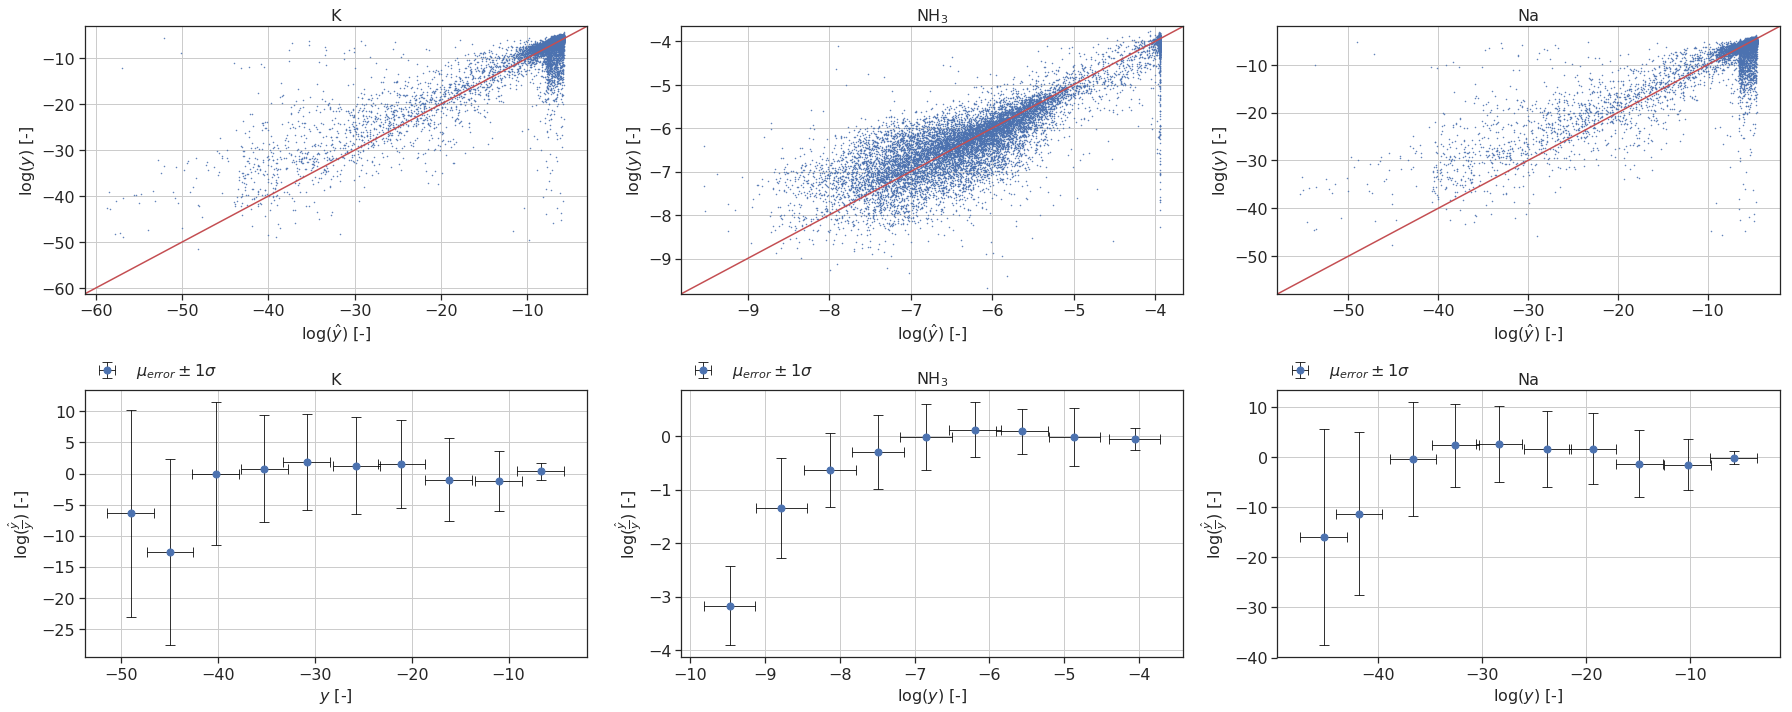
\includegraphics[width=\textwidth,keepaspectratio]{figuren/results4.png}
    \caption{Same as Figure \ref{fig:complex_results_1}.}
    \label{fig:complex_results_4}
\end{figure}

\begin{figure} [!htb]
    \centering
    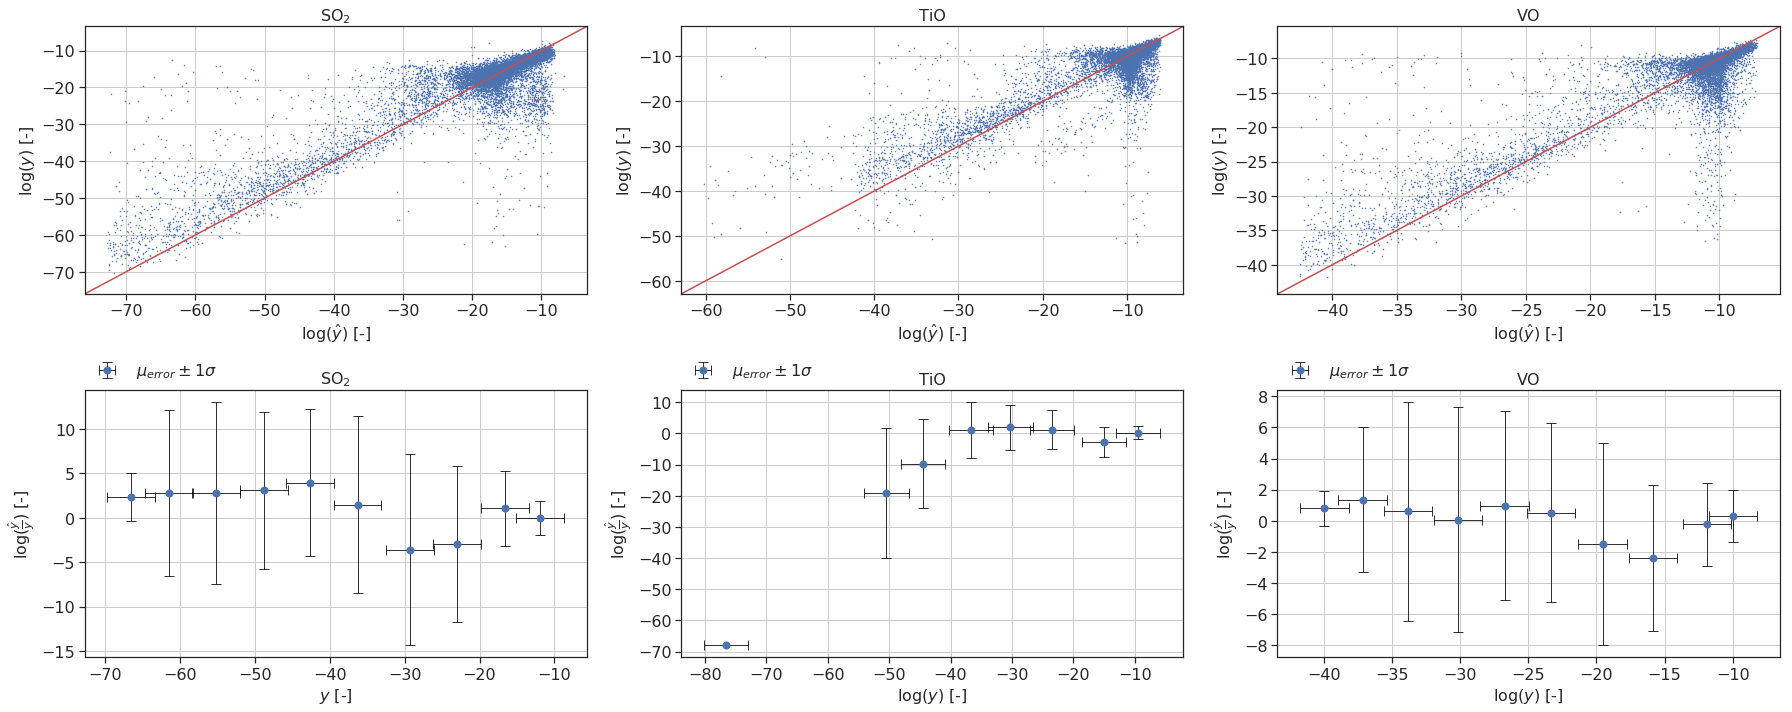
\includegraphics[width=\textwidth,keepaspectratio]{figuren/results5.png}
    \caption{Same as Figure \ref{fig:complex_results_1}.}
    \label{fig:complex_results_5}
\end{figure}

\begin{figure} [!htb]
    \centering
    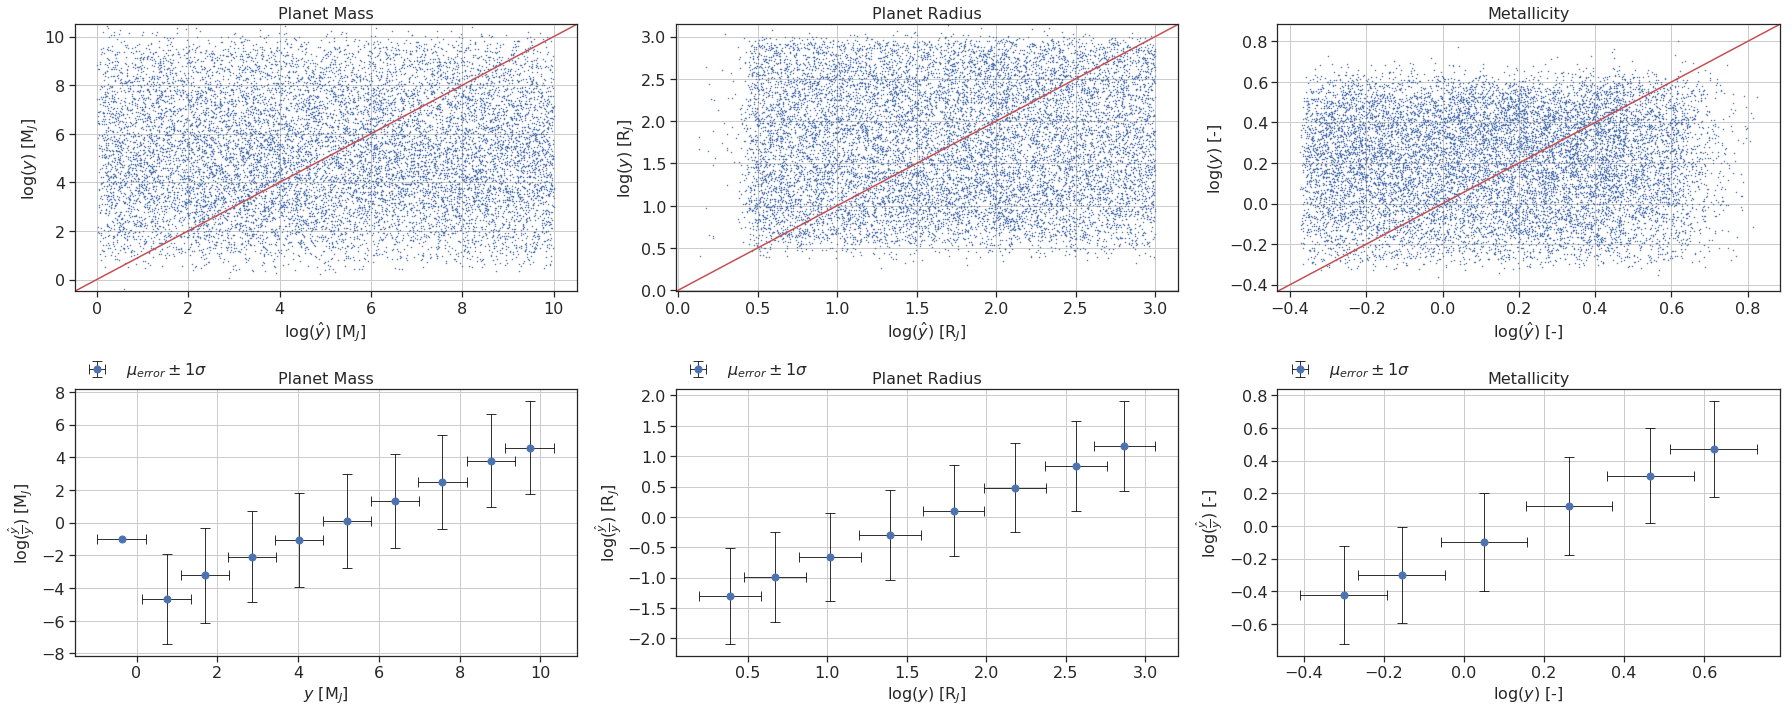
\includegraphics[width=\textwidth,keepaspectratio]{figuren/results6.png}
    \caption{Same as Figure \ref{fig:complex_results_1}.}
    \label{fig:complex_results_6}
\end{figure}

\begin{figure} [!htb]
    \centering
    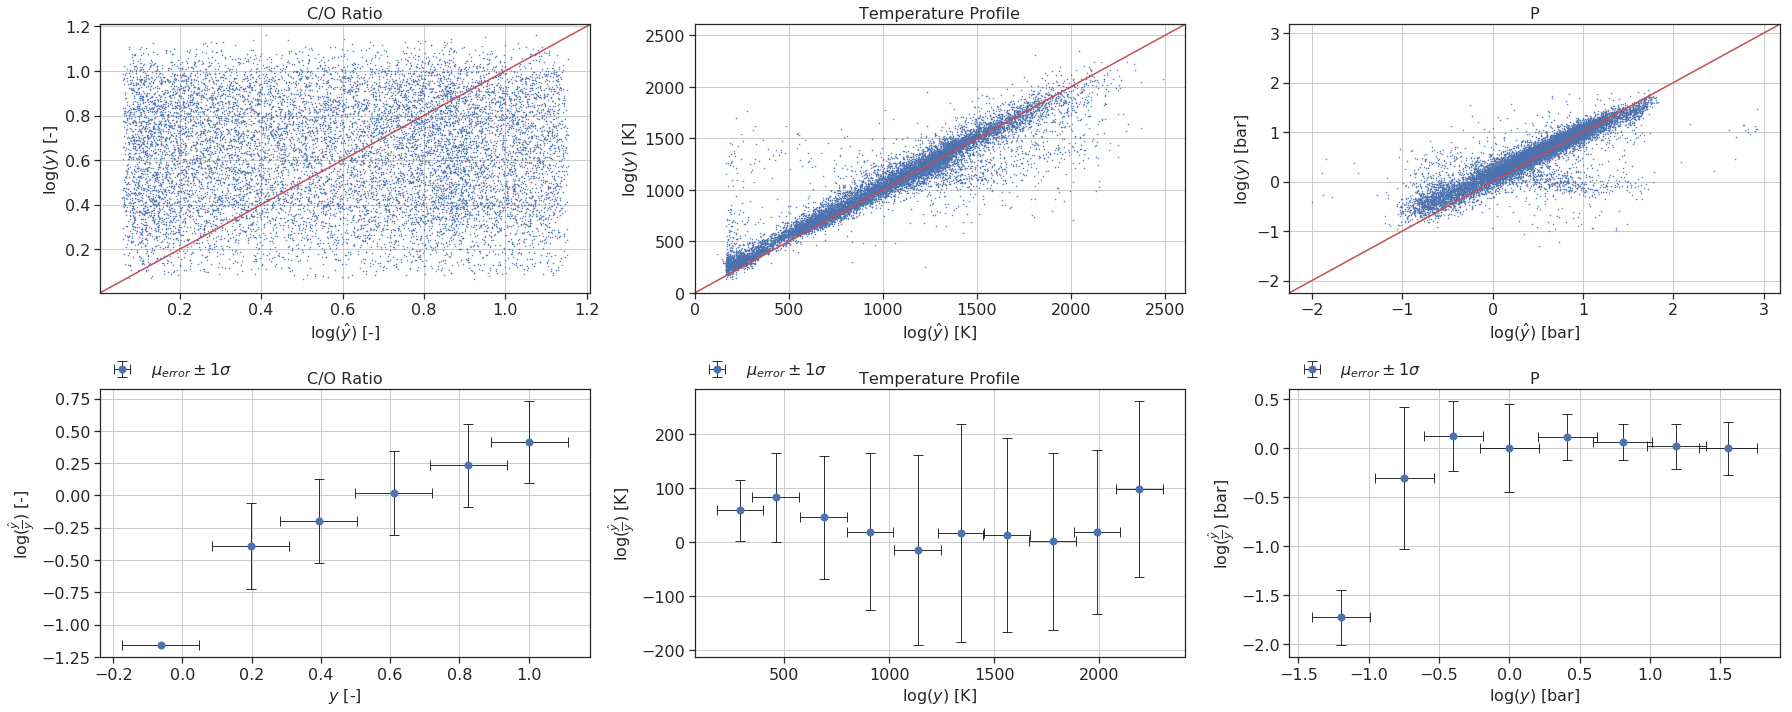
\includegraphics[width=\textwidth,keepaspectratio]{figuren/results7.png}
    \caption{Same as Figure \ref{fig:complex_results_1}.}
    \label{fig:complex_results_7}
\end{figure}

\begin{figure} [!htb]
    \centering
    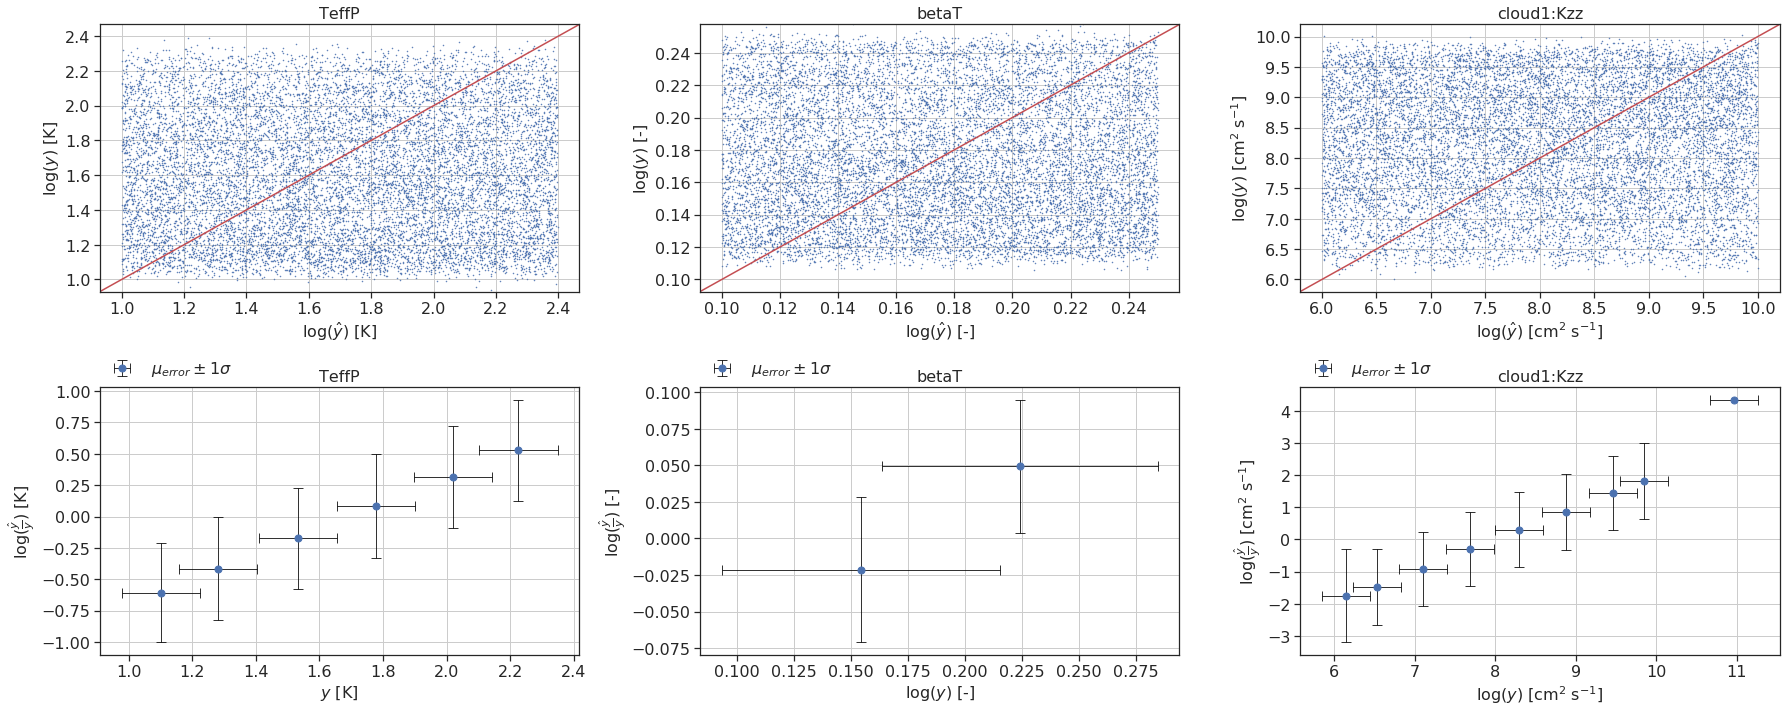
\includegraphics[width=\textwidth,keepaspectratio]{figuren/results8.png}
    \caption{Same as Figure \ref{fig:complex_results_1}.}
    \label{fig:complex_results_8}
\end{figure}

\begin{figure} [!htb]
    \centering
    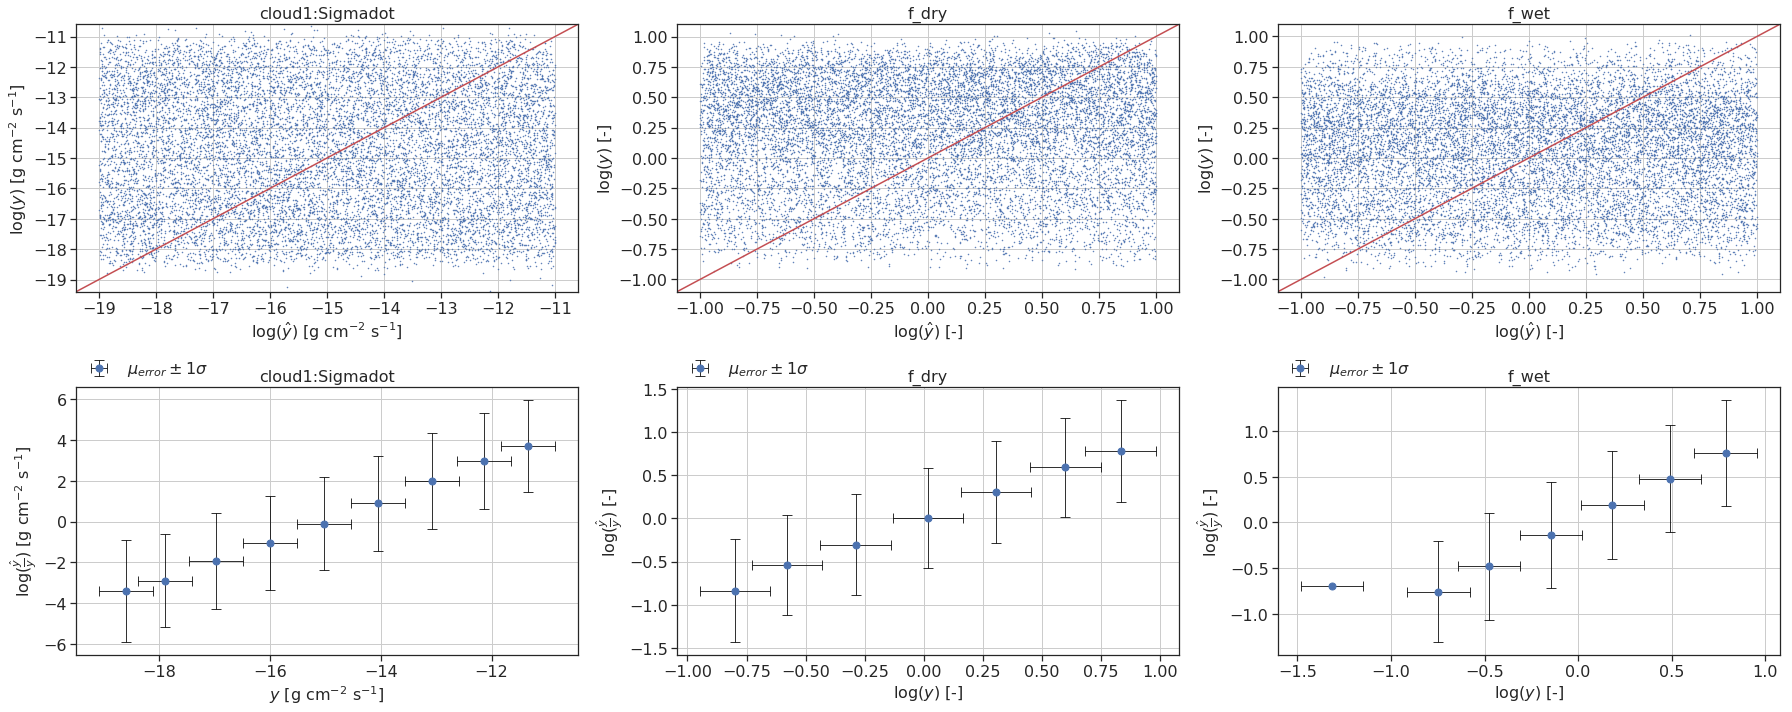
\includegraphics[width=\textwidth,keepaspectratio]{figuren/results9.png}
    \caption{Same as Figure \ref{fig:complex_results_1}.}
    \label{fig:complex_results_9}
\end{figure}

\begin{figure} [!htb]
    \centering
    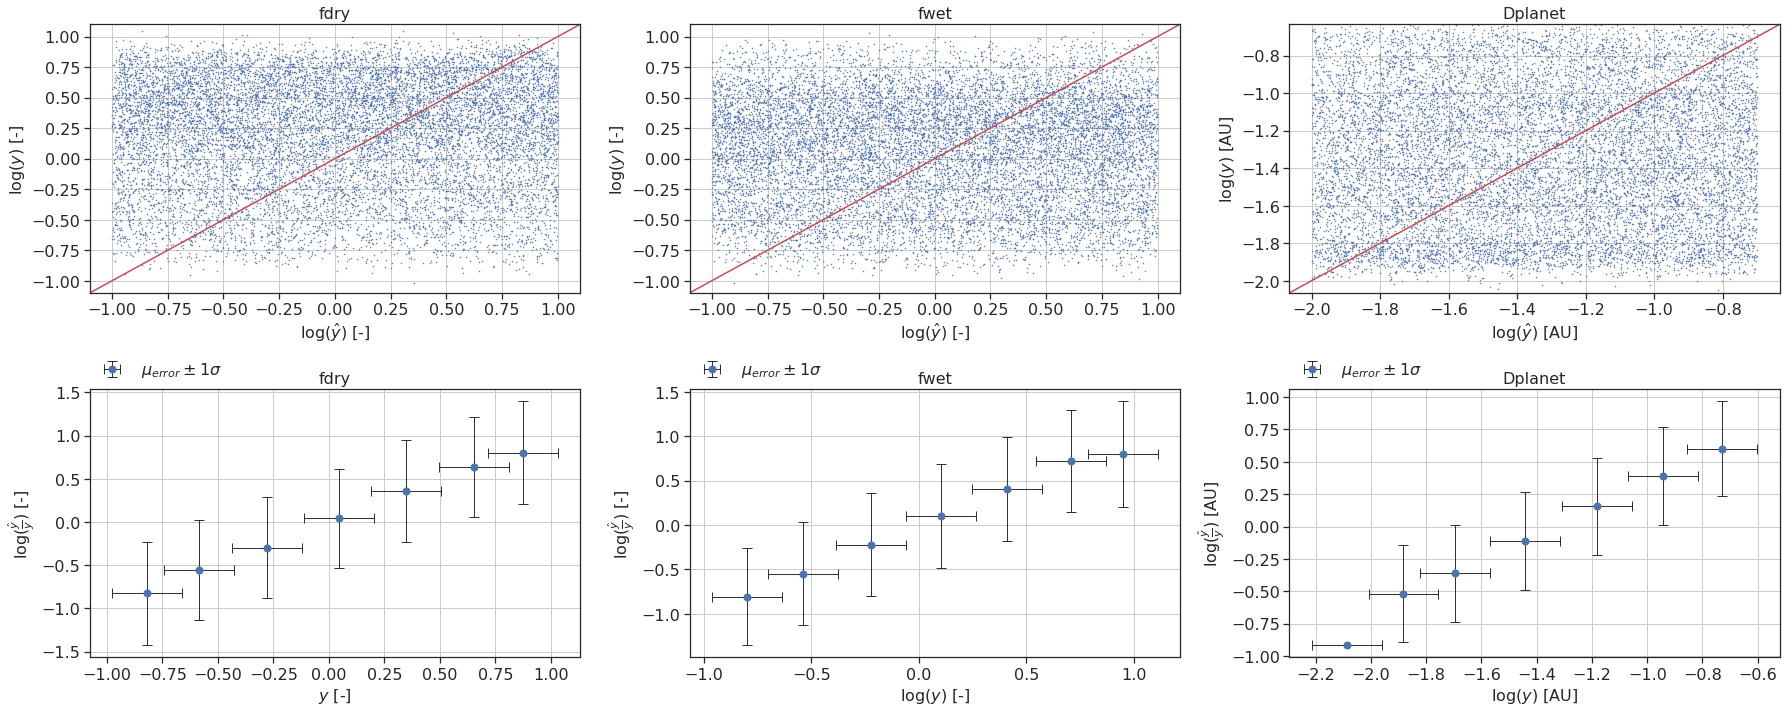
\includegraphics[width=\textwidth,keepaspectratio]{figuren/results10.png}
    \caption{Same as Figure \ref{fig:complex_results_1}.}
    \label{fig:complex_results_10}
\end{figure}






